\documentclass[12pt,letterpaper]{article} 
\usepackage[letterpaper,margin=1in]{geometry} 
\usepackage{mathptmx}
\usepackage[singlespacing]{setspace}
\usepackage{fancyhdr}
\setlength{\headheight}{14.49998pt}
\usepackage{relsize}
\usepackage[bottom]{footmisc}
\usepackage{tabularx}
\setlength{\parindent}{2em}
\usepackage{url}
\usepackage{hyperref}
\usepackage[english]{babel}
\usepackage{graphicx}
\usepackage{booktabs}
\usepackage{natbib}
\usepackage{expex}
\usepackage{amsfonts} 
\usepackage{tikz}
\bibpunct[:]{(}{)}{;}{a}{}{,}
\usepackage{bibentry}
\usepackage{acronym}
\usepackage{multicol}
\author{Ruben Triwari}
\usepackage{scrhack} 
\usepackage{microtype}
\usepackage[acronym,xindy,toc]{glossaries}
\makeglossaries
\loadglsentries{glossary.tex}
\usepackage{ragged2e}
\babelhyphenation[english]{
an-oth-er
ex-am-ple
}
\newtheorem{definition}{Definition}
\newtheorem{example}{Example}[section]
\usepackage{dcolumn}
\newcolumntype{2}{D{.}{}{2.0}}
\usetikzlibrary{
  automata, positioning,
  arrows, matrix, decorations.pathreplacing,
  shapes.geometric
}

\tikzset{ 
  table/.style={
    matrix of math nodes,
    row sep=-\pgflinewidth,
    column sep=-\pgflinewidth,
    nodes={rectangle,text width=3em,align=center},
    text depth=1.25ex,
    text height=2.5ex,
    nodes in empty cells,
    left delimiter=[,
    right delimiter={]},
    ampersand replacement=\&
  }
}

\begin{document}

\begin{center}\uppercase{Ludwig-Maximilians-Universität München}\end{center}
\begin{center}\uppercase{Chair of Theoretical Computer Science and Theorem Proving}\end{center}

\vspace*{10mm}
\begin{center}

\includegraphics[height=40mm]{sigillum.png}
\end{center}
\vspace*{10mm}

\title{Formal Languages and Automatas}
\date{\vspace{-3ex}}
{\let\newpage\relax\maketitle}
\thispagestyle{empty}

\begin{center}
\begin{large}
\begin{Large}
Seminar Paper on Formal Languages and Automatas\\
\end{Large}
for the course ``Algebra \& Computer Science'' \\
\end{large}
\end{center}
\vspace{1cm}
\begin{center}
\begin{large}
Supervisor: Prof. Dr. Jasmin Blanchette\\
\end{large}
\end{center}
\begin{center}
\begin{large}
Advisor: Xavier Genereux\\
\end{large}
\end{center}


\begin{center}
\begin{large}
Submission Date: \date{\today} \\
\end{large}
\end{center}

\vspace{1,5cm}
\cleardoublepage{}
\thispagestyle{empty}
\vspace*{0.8\textheight}
\noindent
\makeatletter
\begin{center}
{\normalfont\bfseries} Disclaimer
\end{center}
\begin{flushleft}
I confirm that this seminar paper is my own work and I have documented all sources and material used.\\
\makeatother
\vspace{15mm}
\noindent
Munich, \date{\today} \hspace{50mm} Author
\end{flushleft}
\cleardoublepage{}


\section*{Abstract}
Abstract...
\textbf{Keywords}: Math

\newpage
\tableofcontents
\newpage

\setcounter{page}{1}
\pagestyle{fancy}
\fancyhf{}
\fancyhead[R]{\thepage}
\renewcommand{\headrulewidth}{0pt} %obere Trennlinie

\section{Introduction}
\section{Backround}
First of all, we need to define some simple structures and ideas,
that will be really important in this paper. We will define 
formal languages in two ways and then automatas arcordingly.
A formal language is just a set of words, where words are 
a series of characters from an alphabet.
\begin{definition}
  An Alphabet is an abritrary non empty finite set denoted with $\Sigma$
\end{definition}
\begin{example} Simple examples for Alphabets would be:
  \begin{enumerate}
    \item $\Sigma = \{x\}$
    \item $\Sigma = \{a,b,c,d, \dots z \}$
    \item $\Sigma = \{1,2,3, \dots n \}$ where $n \in \mathbb{N}$
  \end{enumerate}
\end{example}
This definition is rather general, because an alphabet $\Sigma$
can really be anything. We could also define an Alphabet as subset of
the natural numbers $\Sigma \subset \mathbb{N}$. This is equalivant to
the previous definition, becaus we can always find an isomorphism between
a finite amount of objects and the natural numbers. In other words 
we can always just number a finite amount of objects. The above definition
results in more readable words, thus resulting in more readable problems.
Furhtermore its unintuitive to have words full of numbers and languages
full of number series. That is why im chosing this definition, like most
of the literature.\\
Now with our first building block defined we can define words, which are just
a series of characters in an alphabet.
\begin{definition}
  Let $\Sigma$ be an fixed alphabet, then $w$ is a series of characters out of
  $\Sigma$. The empty words which contains no characters, 
  is denoted by $\epsilon$
\end{definition}
\begin{example}
  Simple examples for words would be:
  \begin{enumerate}
    \item $\Sigma = \{a,b,c\} \rightsquigarrow w_1 = abc$
    \item $\Sigma = \{x\} \rightsquigarrow w_2 = xxxx$
    \item $\Sigma = \{1,2,3\} \rightsquigarrow w_3 = 112233$
    \item $\Sigma = \{1,2,3\} \rightsquigarrow w_4 = \epsilon$
  \end{enumerate}
\end{example}
The empty word $\epsilon$ is analogous to the empty set in Set theory.
It has a lot uf uses, but one obvious is that now one can define 
a Monoid over words $(M, \cdot, \Sigma, \epsilon)$.
M is a set of words and plus is concetanation of words, then 
$\epsilon$ is the neutral element of the Monoid. Which brings us to
the next definition.
\begin{definition}
  Let $\Sigma$ be an fixed alphabet and  $w$, $v$ words with 
  characters out of $\Sigma$. Then the contenation is defined by:
  \[ w \cdot v := wv\]
  sometimes just written as $wv$. With powers:
  \[ 
    w^n = \underbrace{w\cdot w \cdot \dots w}_{\text{n times}}
    \text{ where } n \in \mathbb{N}
  \]
\end{definition}
In simple terms a concatenation of two words is just a new word with 
the two words chained togehter.\\
Now we can again build on words to define langauges.
\begin{definition}
  Let $\Sigma$ be an fixed alphabet, then a formal language is a 
  set of words, with characters in $\Sigma$.
\end{definition}
\begin{example}
  Simple examples for formal languages would be:
  \begin{enumerate}
    \item $\Sigma = \{a,b,c\} \rightsquigarrow L = \{aaa, bbb, ccc, abc\}$
    \item $\Sigma = \{x\} \rightsquigarrow L = \{ x, xx, xxx, xxxx\}$
    \item $\Sigma = \{1,2,3\} \rightsquigarrow L = \{11, 22, 33, 123,\epsilon\}$
  \end{enumerate}
\end{example}
This definition is really clear and simple. We will see a less intuitive way to
define language shortly. Obviously the simpler one has some downsides, 
which we will discuss later in the paper. \\
The kleene star $^*$ is a really powerful operator, to define it we need
to first define contenation for languages.
\begin{definition}
  Let $\Sigma$ be an fixed alphabet and  $L$, $V$ languages with 
  words constructed out of $\Sigma$.
  Then the contenation of formal languages is defined by:
  \[ L \cdot V := \{ l \cdot v | l \in L \lor v \in V \}\]
  sometimes just written as $LV$. With powers defined recursively:
  \begin{align*}
      L^0 & := \{\epsilon \}\\
      L^1 & := L  \\
      L^{i+1} & := \{ l_i\cdot l | l_i \in L^i \lor l \in L\}
  \end{align*}
  % wikipedia kleene star
\end{definition}
In simple terms we are creating a new language by compbining every word
of the first language with every word of the second.
Now we are able to define the kleene star operator.
\begin{definition}
  Let $\Sigma$ be an fixed alphabet and  $L$  a language with 
  words constructed out of $\Sigma$.
  Then the kleene star of  a formal language is defined by:
  \[ 
    L^* := \bigcup_{i \in \mathbb{N}_0} L^i = 
    L^0 \cup L^1 \cup L^2 \cup \dots
  \]
\end{definition}
In simple terms it generates all possible permutation of abriatary length
of a formal language. This is really powerful, because $\Sigma^*$ is the
biggest language one can construct from the alphabet $\Sigma$. Thus every 
language $L$ generated by $\Sigma$ is just a subset of $\Sigma^*$.\\
Unintuively, we can also write a formal language as a formal power series.
\begin{definition}
  Let $\Sigma$ be an fixed alphabet, then a formal language can be 
  written as:
  \[
    L = \sum_{w \in \Sigma^*} (L,w)w \verb| where | 
    (L,w) \in \mathbb{B} = \{0,1\}
  \]
\end{definition}
The sum is iterating over all possible words $w \in \Sigma^*$ and 
$(L,w)$ is an indicating function, which is one if $w$ should be in the
language and ohterwise zero. Thus all words with an one infront are in 
the language.\\
The representation with sets has the andvantage that a formal language
will inherit all operations on sets like complement, union, and intersection.
Those operations are really useful, thus we will define similar on the power
series version.
\begin{definition}
  Let $\Sigma$ be an fixed alphabet $L, V$ formal languages,
  L and V can be written
  \[
    L = \sum_{w \in \Sigma^*} (L,w)w \hspace{0.5cm} \text{and} \hspace{0.5cm}
    V = \sum_{w \in \Sigma^*} (V,w)w.
  \]
  Addition and multiplication on formal power series is defined
  as follows:\\
  \[
    L + V := \sum_{w \in \Sigma^*} ((L,w) + (V,w))w
    \hspace{0.5cm} \text{and} \hspace{0.5cm} 
    L \cdot V := \sum_{w \in \Sigma^*} ((L,u) \cdot (V,v))w
    \verb|,|\hspace{0.5cm} \verb|where | w = uv.
  \]
  This definition is not recursive, because the right addition and 
  muliplication operater are from the Boolean Algebra 
  $\mathbb{B} = \{0,1\}$.
  \begin{center}
    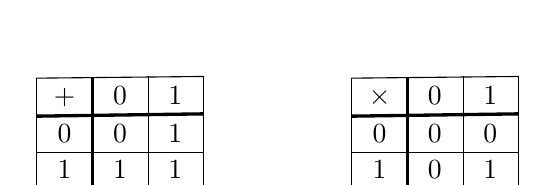
\begin{tikzpicture}
      \matrix (m) [nodes={minimum width=2em,minimum height=2ex},matrix of nodes]
      {
      $+$&0&1\\
      0&0&1\\
      1&1&1\\
      };
      \draw[very thick] (m-1-1.north east) -- (m-3-1.south east);
      \draw[very thick] (m-1-1.south west) -- (m-1-3.south east);
      \draw (m-1-1.north west) -- (m-3-1.south west);
      \draw (m-1-1.north west) -- (m-1-3.north east);
      \foreach \x in {2,...,3}{
        \draw (m-1-\x.north east) -- (m-3-\x.south east);
        \draw (m-\x-1.south west) -- (m-\x-3.south east);
      }

      \matrix [
        nodes={minimum width=2em,minimum height=2ex}
        ,matrix of nodes
      ] at (4,0)
      {
        \node(a){$\times$}; & \node(b){0}; & \node(c){1}; \\
        \node(d){0}; & \node(e){0}; & \node(f){0}; \\
        \node(g){1}; & \node(h){0}; & \node(i){1};\\
      };
      \draw[very thick] (a.south west) -- (c.south east);
      \draw[very thick] (a.north east) -- (g.south east);

      \draw (a.north west) -- (c.north east);
      \draw (a.north west) -- (g.south west);

      \draw (b.north east) -- (h.south east);
      \draw (d.south west) -- (f.south east);

      \draw (c.north east) -- (i.south east);
      \draw (g.south west) -- (i.south east);

    \end{tikzpicture}
  \end{center}
  With powers defined recursively:
  \begin{align*}
    L^0 &:= \epsilon\\
    L^1 &:= L\\
    L^{i+1} &:= \sum_{w \in \Sigma^*} ((L^i,u)\cdot (L,v))w, 
    \hspace{0.5cm} \text{where} \hspace{0.5cm} w = uv.
  \end{align*}
  Kleene Star can now also be defined for formal power series:
  \[
    L^* := L^0 + L^1 + L^2 + L^3 + \dots = \sum_{i \in \mathbb{N}_0} L^i.
  \]
\end{definition}
With these operation defined our two versions of formal languages are 
powerful tools, which will be compared in the following sections. In order
to conpare them we will also need finite automatas. Simillar to formal languages
there are multiple ways one can define finite automatas. In this paper we
will define two. One is more suitable for combining it with the set version
of formal languages and the other one is more siutable for the formal power
series representation. First we will define the one more suitable for the
set version.
\begin{definition}
  A finite automata is a quintuple $M = (Q, \Sigma, \delta, q_0, F)$, 
  where
  \begin{enumerate}
    \item Q is a finite set of states,
    \item $\Sigma$ is an alphabet, all inputs are constructed from,
    \item $\delta: Q \times \Sigma \to Q$ is the transition function,
      carrying the automata from one state to another,
    \item $q_0 \in Q$ is the initial state of the automata,
    \item $F \subset Q$ are the accepting states of the automata.
  \end{enumerate}
  %Definition is out of theoretical computer science book (german)
\end{definition}
\begin{example}
  Here is a simple automata depicted, where the circles are states
  , the arrows are transitions, the start is indicating the initial 
  state, and the double lined circle is the accepting state.
  $M = ()$
    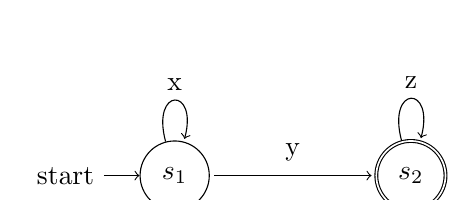
\begin{tikzpicture}
      \node[state,initial] (q1) at (0,0) {$s_1$};
      \node[state,accepting] (q2) at (3,0) {$s_2$};
      \draw (q1) edge[loop above] node{x} (q1)
      (q2) edge[loop above] node{z} (q2);
      \draw[->](0.5,0)--(2.5,0);
      \node[fill=white] at (1.5,0.3) {y};
    \end{tikzpicture}
\end{example}









% Define Formal languages (Sets and Power sereies) 
% and automatas (Tuple and Matrix)
\section{Formal Languages: Sets vs. Formal Power Series}
% translate one in another
% Formal power series are an algebra over Boolean algebra
% U could define the same algebra for sets with set operations
% But u could replace the boolean algebra by any abritary ring
% Which makes formal power series more powerful cuz u can abstract even more
\section{Maximum Gap Lemma}
\section{Pumping Lemma}
\section{Not all Formal languages are regular}
\section{Pumping Lemma vs. Maximum Gap Lemma}
\section{Kleene's theorem (Power series, Matrix Automata)}
\section{Kleene's theorem (Set, Tuple)}
\section{Kleene's theorem vs. Kleene's theorem}
\section{Kleene Schützenberg theorem and weigthed automatas}
\section{Conclusion}


\subsection{Citation} 
\label{sec:cit}

The citation method follows the author-year system. Place reference is in the text, footnotes should only be used for explanations and comments. The following notes are taken from the \emph{language} bibliography template from \url{ron.artstein.org}:\newline

\noindent
The \emph{Language} style sheet makes a distinction between two kinds of in-text citations: citing a work and citing an author.
\begin{itemize}
\item Citing a work:
  \begin{itemize}
    \setlength{\itemsep}{0pt}
    \setlength{\parsep}{0pt}
  \item Two authors are joined by an ampersand (\&).
  \item More than two authors are abbreviated with \emph{et al.}
  \item No parentheses are placed around the year (though parentheses
    may contain the whole citation). 
  \end{itemize}
\item Citing an author:
  \begin{itemize}
    \setlength{\itemsep}{0pt}
    \setlength{\parsep}{0pt}
  \item Two authors are joined by \emph{and}.
  \item More than two authors are abbreviated with \emph{and colleagues}.
  \item The year is surrounded by parentheses (with page numbers, if
    present).
  \end{itemize} 
\end{itemize}
To provide for both kinds of citations, \verb+language.bst+ capitalizes on the fact that \verb+natbib+ citation commands come in
two flavors. In a typical style compatible with \verb+natbib+, ordinary commands such as \verb+\citet+ and \verb+\citep+ produce short
citations abbreviated with \emph{et al.}, whereas starred commands such as \verb+\citet*+ and \verb+\citep*+ produce a citation with a
full author list. Since \emph{Language} does not require citations with full authors, the style \verb+language.bst+ repurposes the starred commands to be used for citing the author. The following table shows how the \verb+natbib+ citation commands work with \verb+language.bst+.
\begin{center}
  \begin{tabular}{lll}
    \toprule
    Command & Two authors & More than two authors \\
    \midrule
    \verb+\citet+ & \citet{hale} & \citet{sprouse} \\
    \verb+\citet*+ & \citet*{hale} & \citet*{sprouse} \\
    \addlinespace
    \verb+\citep+ & \citep{hale} & \citep{sprouse} \\
    \verb+\citep*+ & \citep*{hale} & \citep*{sprouse} \\
    \addlinespace
    \verb+\citealt+ & \citealt{hale} & \citealt{sprouse} \\
    \verb+\citealt*+ & \citealt*{hale} & \citealt*{sprouse} \\
    \addlinespace
    \verb+\citealp+ & \citealp{hale} & \citealp{sprouse} \\
    \verb+\citealp*+ & \citealp*{hale} & \citealp*{sprouse} \\
    \addlinespace
    \verb+\citeauthor+ & \citeauthor{hale} & \citeauthor{sprouse} \\
    \verb+\citeauthor*+ & \citeauthor*{hale} & \citeauthor*{sprouse} \\
    \verb+\citefullauthor+ & \citefullauthor{hale} & \citefullauthor{sprouse} \\
    \bottomrule
  \end{tabular}
\end{center}
Authors of \emph{Language} articles would typically use \verb+\citet*+, \verb+\citep+, \verb+\citealt+ and \verb+\citeauthor*+, though they
could use any of the above commands. There is no command for giving a full list of authors.

\subsection{Bibliography}
The bibliography of this template includes the references of the \emph{language} stylesheet as a sample bibliography.


\pagebreak

\microtypesetup{protrusion=false}
\listoffigures{}
\listoftables{}
\microtypesetup{protrusion=true}

\clearpage
\printglossaries
\pagebreak
\addcontentsline{toc}{section}{Bibliography}
\pagestyle{fancy}
\bibliographystyle{language-dt} 
\bibliography{bibliography} 
\nocite{*}
\end{document}
